\chapter{Background on Storm}

In this chapter we give background information on Storm. This information is necessary to understand the design of Storm-MC. We give a quick overview of Apache Storm (\ref{sec:storm_overview}), explain the concepts used in Storm (\ref{sec:concepts}), show an example Storm program (\ref{sec:example_topology}), give details about the underlying architecture of Storm (\ref{sec:storm_arch}), and finally describe the serialisation used in Storm (\ref{sec:serialisation}).

\section{Storm Overview}
\label{sec:storm_overview}

Apache Storm was developed in a mix of Java and Clojure. As mentioned by the author of Storm in \cite{Marz_2014}, writing the Storm interfaces in Java ensured large potential user-base while writing the implementation in Clojure increased productivity.

To ensure API compatibility with Storm, Storm-MC was developed using the same set of languages. This allowed for code reuse and not having to re-implement functionality already present in Storm. Hence, in the following sections we describe Storm in greater detail in hope that this will later clarify design choices made for Storm-MC.

\section{Storm Concepts}
\label{sec:concepts}

\subsection{Core Concepts}

There are several core concepts used by Storm and hence by extension Storm-MC as well. These concepts are put together to form a simple API that allows the programmer to break down a computation into separate components and define how these components interact with each other. The three core concepts of Storm are:

\begin{description}
  \item[Spout] \hfill \\
  A spout is a component that represents the source of a data-stream. Typically, a spout reads from a message broker such as RabbitMQ \cite{RabbitMQ} or Apache Kafka but can also generate its own stream or read from somewhere like the Twitter streaming API \citep{TwitterStreaming}.
  \item[Bolt] \hfill \\
  A bolt is a component that transforms tuples from its input data stream and emits them to its output data stream. A bolt can perform a range of functions e.g. filter out tuples based on some criteria or perform a join of two different input streams.
  \item[Topology] \hfill \\
  The programmer connects spouts and bolts in a directed graph called topology which describes how the components interact with each other. The topology is then submitted to Storm for execution.
\end{description}

Every component is represented by a set of tasks. These tasks can run in parallel and execute the function of the component.

It should also be noted that spouts and bolts can be implemented not only in Java but other languages such as Python and Ruby.

\subsection{Additional Concepts}

There are several additional concepts which describe how components of a topology interact:

\begin{description}
  \item[Stream] \hfill \\
  A stream is defined as an unbounded sequence of tuples. Streams can be thought of as edges of a topology connecting bolts and spouts (vertices).
  \item[Tuple] \hfill \\
  A tuple wraps named fields and their values. The values of the fields can be of different types. When a component emits a tuple to a stream it sends that tuple to every bolt subscribed to the stream.
  \item[Stream Grouping] \hfill \\
  Every bolt needs to have a type of stream grouping associated with it. This grouping decides the means of distributing the tuples coming from a bolt's input stream among task instances of the bolt. Following are the possible types of stream grouping:
  \begin{description}
  	\item[Shuffle] Randomly partition the tuples among all the bolt tasks.
  	\item[Fields] Hash on a subset of the tuple fields. All tuples with same values of those fields will go to same bolt task.
  	\item[All] Replicate the entire stream to all the bolt tasks.
  	\item[Direct] The producer of the tuple decides which task of the bolt will receive this tuple.
  	\item[Global] Send the entire stream to a single bolt task.
  	\item[Local or Shuffle] Prefer sending to tasks in the same node, if that is not possible use same strategy as Shuffle.
  \end{description}
\end{description}

Users are also able to specify their own custom grouping by implementing the \texttt{CustomStreamGrouping} interface.

All the components of a Storm topology execute in parallel. The user can specify how much parallelism he wants associated with every component and Storm spawns the necessary number of threads. This is done through a configuration file, defined in YAML, which is then submitted along with the topology.

There are two additional bolts running for every topology:

\begin{description}
	\item[Acker] \hfill \\
	The Acker bolt guarantees fault tolerance for the topology. It tracks every tuple that was produced and ensures that the tuple has been acknowledged by every bolt of the stream.
	\item[System Bolt] \hfill \\
	The System bolt is useful in two ways:
	\begin{description}
		\item[Metrics] System bolt collects metrics on the local Java Virtual Machine (JVM). Other components can subscribe to these metrics and receive their values at  regular intervals.
		\item[Ticks] Components of a topology can subscribe to receive tick tuples in regular intervals. These tuples can be used to trigger events at subscribed components.
	\end{description}
\end{description}

\section{Example Topology}
\label{sec:example_topology}

\begin{figure}[!htb]
	\centering
	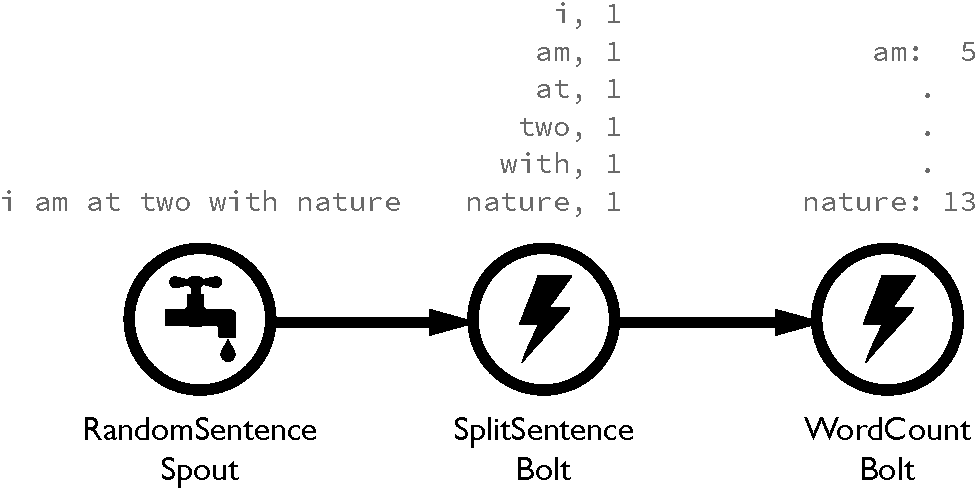
\includegraphics[scale=0.475]{pdf/wordcount_topology.pdf}
	\caption{WordCount topology.}
	\label{fig:wordcount_topology}
\end{figure}

A classic example used to explain Storm topologies is the WordCount topology. In this topology, there is a spout generating random sentences, a bolt splitting the sentences on white space, and a bolt counting occurrences of every word. Figure \ref{fig:wordcount_topology} shows how we could represent this topology graphically.

This may seem as a simplistic example but it is useful when demonstrating how easy it is to implement a working topology using the Storm API.

Listing \ref{listing:wordcount_topology} shows how the topology is put together in Storm to form a graph of components. Storm uses the Builder design pattern \citep{gamma1994design} to build the topology which is then submitted to an emulated cluster for execution. The last argument to the~\texttt{setBolt}/\texttt{setSpout} method is the number of parallel tasks we want Storm to execute for the respective component. For implementation of the spout and the bolts used in this topology, refer to Appendix \ref{ch:listings}.

\begin{listing}[!htb]
\inputminted{java}{code/WordCountTopology.java}
\caption{WordCountTopology.java}
\label{listing:wordcount_topology}
\end{listing}

\section{Storm Architecture}
\label{sec:storm_arch}

\begin{figure}[!htb]
	\centering
	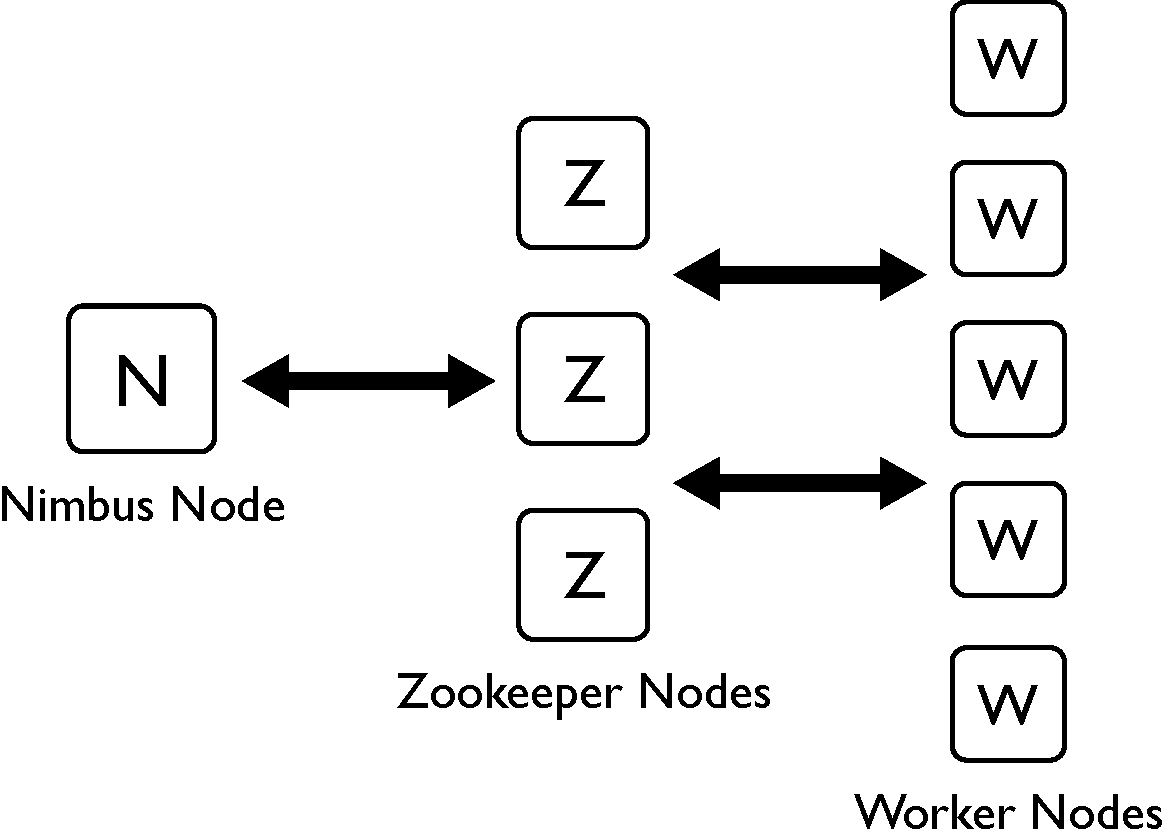
\includegraphics[scale=0.4]{pdf/storm_arch.pdf}
	\caption{Apache Storm architecture.}
	\label{fig:storm_arch}
\end{figure}

%\todo{Maybe highlight similarities to Hadoop}

A Storm cluster adopts the Master-Worker pattern. To set up a Storm topology, the user launches daemon processes on nodes of the cluster and submits the topology to the master node, also called Nimbus. The worker nodes receive task assignments from the master and execute the tasks assigned to them. The coordination between the master node and the worker nodes is handled by nodes running Apache Zookeeper. Figure \ref{fig:storm_arch} shows a graphical representation of Storm architecture.

\subsection{Nimbus Node}

The master node runs a server daemon called Nimbus. The main role of Nimbus is to receive topology submissions from clients. Upon receiving a topology submission, Nimbus takes the following steps:

\begin{description}
	\item[Validate the topology] \hfill \\
	The topology is validated using a validator to ensure the submitted topology is valid before trying to execute it. Programmers using Storm can write their own validator by implementing the \texttt{ITopologyValidator} interface.
	\item[Distribute the topology source code] \hfill \\
	Nimbus ensures that the workers involved in the topology computation have the source code by sending it to all nodes of the cluster.
	\item[Schedule the topology] \hfill \\
	Nimbus runs a scheduler that distributes the work among workers of the cluster. Similarly to validation, the user can use his own scheduler by implementing the \texttt{IScheduler} interface or use the default scheduler provided by Storm. The default scheduler uses a simple Round-robin strategy \citep{Aniello_Baldoni_Querzoni_2013}.
	\item[Activate the topology] \hfill \\
	Nimbus transitions the topology to active state which tells the worker nodes to start executing it.
	\item[Monitor the topology] \hfill \\
	Nimbus continues to monitor the topology by reading heartbeats sent by the worker nodes to ensure that the topology is executing as expected and worker nodes have not failed.
\end{description}


Nimbus is an Apache Thrift \cite{ApacheThrift} service (more on Thrift in section \ref{sec:serialisation}) that listens to commands submitted by clients and modifies the state of a cluster accordingly. Following are the commands supported by Nimbus:

\begin{description}
	\item[Submit a topology] \hfill \\
	Clients can submit a topology defined in a Java Archive (JAR) file. The Nimbus service then ensures that the topology configuration and resources are distributed across the cluster and starts executing the topology as previously described.
	\item[Kill a topology] \hfill \\
	Nimbus can stop running a topology and remove it from the cluster. However, the cluster can still continue executing other topologies.
	\item[Activate/deactivate a topology] \hfill \\
	Topologies can be deactivated and reactivated by Nimbus. This could be useful if the spout temporarily cannot produce a stream and the user does not want the cluster to execute idly.
	\item[Rebalance a topology] \hfill \\
	Nimbus can rebalance a topology across more nodes. Thus if the number of nodes in the cluster ever changes the user can increase or decrease the number of nodes involved in the topology computation.
\end{description}

\subsection{Worker Nodes}

The worker nodes run a daemon called Supervisor. There are 4 layers of abstraction which control the parallelism of a worker node.

\begin{description}
	\item[Supervisor] \hfill \\
	A supervisor is a daemon process the user runs on a worker node to make it part of the cluster. It launches worker processes and assigns them a port they can receive messages on. Furthermore, it monitors the worker processes and restarts them if they fail. A worker node runs only one supervisor process.
	\item[Worker] \hfill \\
	A worker process is assigned a port and listens to tuple messages on a socket associated with the port. A worker launches executor threads as required by the topology. Whenever it receives a tuple, it puts it on a receive queue of the target executor.
	
	Furthermore, the worker has a transfer queue where its executors enqueue tuples ready to be sent downstream. There can be multiple worker processes running inside one supervisor.
	\item[Executor] \hfill \\
	An executor controls the parallelism within a worker process. Every executor runs in a separate thread. An executor's job is to pick up tuples from its receive queue, perform the task of a component it represents, and put the transformed tuples on the transfer queue of the worker. There can be many executors running inside one worker and an executor performs one (the usual case) or more tasks.
	\item[Task] \hfill \\
	A task represents the actual tuple processing function. However, within an executor thread all the tasks are executed sequentially. The main reason for having tasks is that the number of tasks stays the same throughout the lifetime of a topology but the number of executors can change (by rebalancing). Thus if some worker nodes in the cluster go down, the topology can continue executing with the same number of tasks as before.
\end{description}

\subsection{Zookeeper Nodes}
\label{subsec:zookeeper}

A Storm cluster contains a number of Zookeeper nodes which coordinate the communication between Nimbus and the worker nodes. Storm does this by storing the state of the cluster on the Zookeper nodes where both Nimbus and worker nodes can access it.

The cluster state contains worker assignments, information about topologies, and heartbeats sent by the worker nodes to be read by Nimbus. Apart from the cluster state, Storm is completely stateless. Hence, if the master node or a worker node fail the cluster continues executing and the node will get restarted if possible. The only time the cluster stops executing  completely is if all the Zookeper nodes die.

\section{Serialisation}
\label{sec:serialisation}

Since Storm topologies execute on a cluster all components need to be serialisable. This is achieved with Apache Thrift. Components are defined as Thrift objects and Thrift generates all the Java serialisation code automatically.

Furthermore, since Nimbus is a Thrift service Thrift generates all the code required for remote procedure call (RPC) support. This allows defining topologies in any of the languages supported by Thrift and easy cross-language communication with the Nimbus service.

